% !TeX root = vpl.tex

\chap{Changing Colors}\label{ch.colors}

\sect{Display colors}

Create a program that causes two different colors to be displayed on
the top of the Thymio robot when the front and back buttons are
touched, and two other colors to be displayed on the bottom of the robot
when the left and right buttons are touched.

{\raggedleft \hfill Program file \bu{colors.aesl}}

We need four event-action pairs.
There are four events---touching the
four buttons---and a color action is associated with each event. Note the
difference between the action blocks \blksm{action-colors-up-white} and
\blksm{action-colors-down-white}. The first block changes the color
displayed on the top of the robot, while the second changes the color on
the bottom of the robot. The block for the bottom has two black marks
that represent the wheels.

This program is shown in \cref{fig.colors-a}.

What colors are displayed? In the first three actions, the slider for
one color is moved to the right edge and displayed, while the sliders
for the other two colors are moved to the left edge and are not mixed
in. Therefore, these actions display pure red, blue and green,
respectively. The action associated with the left button mixes red and
green giving yellow.
You can see that the background of the color action changes depending on the
sliders' positions; the background shows you which color your Thymio will display.

Run the program (icon \blksm{run}) and check that touching buttons changes the robot's color.
\Cref{fig.front} shows the Thymio displaying red on
the top and \cref{fig.bottom} shows it displaying green on the
bottom.

\exercisebox{\thechapter.1}{
Experiment with the sliders to see which colors can be displayed.
}

\trickbox[Information]{
\gr{color-cubes-en}{1}
By mixing together red, green and blue, you can make any color!
}

\sect{Turn the lights off}

Let us modify the program so that the lights are turned off when the
center button is touched. We need two event-action pairs, one to turn
off the top light and the other to turn off the bottom light.
By moving all three sliders in the color action block to the left, as in \cref{fig.colors-b}, no colors are displayed and the light is turned off.
The \emph{event is the same} in both pairs---touching the center button---but
the \emph{actions are different}---turning off the top or bottom light. 

Do not forget to click on the icon \blksmpure{run} to run the program.
In the future, we will not remind you to click this icon to run a program.

\vfill

\importantbox[Multiple event-action pairs]{
\begin{itemize}[noitemsep,nosep,leftmargin=*]
\item When a program is run, all the event-action pairs in the program
are run.
\item It is possible for several pairs to have the same event as
long as they have different associated action blocks.
\item If the event and the action block are similar in several pairs, VPL will
display an error message (area 3 in \cref{fig.vplgui}).
You will not be able to run the program as long as there are errors.
\end{itemize}
}

\begin{figure}
    \centering
    \subfigure[Changing colors when a button is touched]{
		\label{fig.colors-a}
		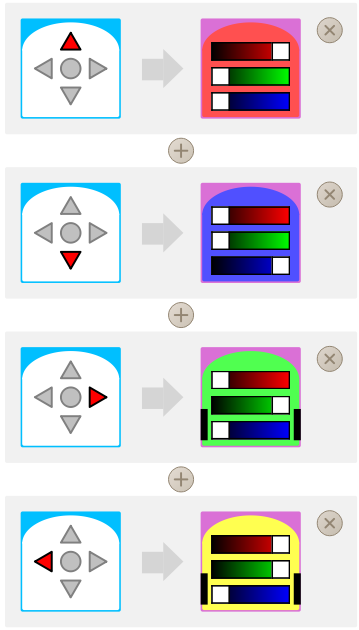
\includegraphics[width = 0.4\textwidth]{colors1}
	}
	\hspace{1.5cm}
    \subfigure[Turn the colored lights off when a button is touched]{
		\label{fig.colors-b}
		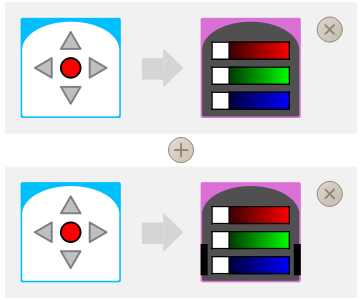
\includegraphics[width = 0.4\textwidth]{colors2}
	}
    \caption{Play with the lights of Thymio}
    \label{fig.colors}
\end{figure}
